\chapter{Visualization}
\label{ch:viz}

While the previous two chapters have focused on algorithmic uses of topic
models, one of the reasons for using topic models is that they produce
human-readable summaries of the themes of large document collections.  However,
for users to use the results of topic models, they must be able to understand
the models' output.  This depends on \emph{visualization} and \emph{interaction}
with the model.

We begin this chapter with a discussion of how best to show individual topics to
users.  From these foundations, we move to how we can display entire
models---with many topics---to users.  Finally, we close with how users can
provide feedback through these interfaces to improve the underlying model.

\section{Displaying Topics}
\label{sec:display}

Recall from the previous chapter that topics are distributions over words; the
words with the highest weight in a topic best explain what the topic is about.
While the simplest answer---just show the most probable words---is a common
solution, there are possible refinements that can improve a user's understanding
of a dataset by showing the relationships between words or explicitly showing
words' probability.

% cite TACL paper
\paragraph{Word Lists}

Just showing a list of the most common words (a
visualization that we'll call ``word list'') is very simple, it also works well.
Users can quickly understand what's going on, and it is an efficient use of
space.  represented horizontally~\cite{gardner2010topic,smith2015visual} or
vertically~\cite{eisenstein2012topicviz,chaney2012visualizing}, with or without
commas separating the individual words, or using set
notation~\cite{chaney2012visualizing}.  \citet{smith2015visual} go further by
adding bars representing the probabilities of the word.

\paragraph{Word Clouds}

Word clouds (e.g., Figure~\ref{fig:word-cloud}) are another popular approach for
displaying topics.  Unlike word lists, they also use the size of words to convey
additional information. Word clouds typically use the size of words to reflect
the probability of the words.  This uses more of a given visualization area to
be used to display a topic.

However, word clouds have been criticized for providing poor support for visual
search~\cite{Viegas2008} and lacking contextual information between
words~\cite{harris11}; users can sometimes draw false connections between words
that are placed next to each other randomly in a word cloud.  Another
alternative is to use word associations to layout
words~\citep{Smith:Chuang:Hu:Boyd-Graber:Findlater-2014};
Figure~\ref{fig:topic-in-a-box} shows places words that appear together next to
each other in the visualization.

\subsection{When Words aren't Enough}

Multi-word expressions can be discovered through
pre-processing~\citep{talley-11}, post-processing step~\citep{blei-09b},
or a joint model~\citep{johnson-10}.

\section{Labeling Topics}

Throughout this survey, we've been referring to topics about
\underline{information technology} or about \underline{the arts}.  These are
convenient labels, but completely removed from the raw distribution over words.
Thus, it's often useful to assign labels to topics within an interface.

In contrast to the previous \emph{visualization} approaches, labeling
focuses son showing not the original words of a topic but rather a
clearer label more akin to what a human summary of the data would
provide.

Approaches for automatic labeling can be divided into those that only
use internal information from the topic model against those that also
use external knowledge resources.  While purely internal methods are
more robust and consistent with the philosophy of unsupervised topic
models, those that use external resources often produce higher quality
labels.

Of the techniques that use external resources, we further separate
those that use direct supervision for labeling (i.e., knowing what
constitutes a good labeling) from those that use general knowledge
resources such as Wikipedia or knowledge bases.

\paragraph{Internal Labeling}

\citet{mei-07} propose an internal labeling method that takes
prominent phrases from the topic and compares how consistent the
phrase's context is with the topic distribution.  Phrases whose
contexts closely resemble the topic often appear in regions of text
that summarize the document, making them good candidates for labels.
\cite{mao-12} extend the technique to hierarchies, using the insight
that parents’ labels should be consistent with their childrens'.

% What about Tim W at UIUC?

% I didn't really understand this paper: Automatic Labelling of Topic
% Models Learned from Twitter by Summarisation (shoud we cite?)

\paragraph{Labeling with Supervised Labels}

% Frank Wood / Noemi hierarchically supervised model?

\citet{lau-10} use a supervised approach to rerank the words in a
topic to ensure that the „best“ word in the topic is shown to a
user.  Each candidate word forms a feature vector consisting of
features such as the following:
\begin{itemize*}
\item the conditional probability of a word given the other words in a
  topic (which implies topic coherence, as discussed in Section~\ref{});
\item whether the word is a hypernym of other words in the topic
  (e.g., ``dog'' in a topic that also contains ``terrier'' and
  ``poodle''); and
\item the original probability of the word in the topic.
\end{itemize*}

While these can be used alone as an unsupervised reranking,
\citet{lau-10} use user-selected best topic words to weight which of
these features are most important for selecting the best topic word.
These weights are learned using support vector regression~\cite{}.
\citet{lau-11} extend their technique by adding candidates from
Wikipedia to the set and show that models learned on different domain
corpora are still effective.

\paragraph{Labeling with Knowledge Bases}

% Perhaps have a figure to give an example
\citet{mao-12} align topic models with an external ontology of
labels.  They argue that labels should match topic words (as labeling with flat
topics); a topic's words should be consistent with a labels' children in the
hierarchy; and the topic's labels should be unique.

\citet{aleteras-14} instead query the whole web and then build a graph that
includes the words that make up the titles of the retrieved webpages. The edges
between the words is the \abr{npmi} computed on a reference corpus.  The
intuition is that words that are ``central'' in this graph will be a good title
for the topic.  They find the central words by using the PageRank~\citep{page-99}
algorithm.  This finds words that are highly probable in the topic and appears
often with many other words in the topic.

\paragraph{Using Labeled Documents}

The task of associating labels with topics becomes much easier if many of your
documents are themselves labeled.  Labeled \abr{lda}~\citep{ramage-09}
associates topics to each of the labels and forces labeled documents to only use
the topics associated with the document.  This constraint forces the topics to
be consistent with the original labels (Figure~\ref{fig:llda}).
\citet{Bakalov-12} extend this to hierarchical label sets (e.g., \abr{ny} Times
subjects that place \underline{Russia} under \underline{International}), while
\citet{nguyen:boyd-graber:resnik:chang-2014} extend it to learning hierarchies
of topics from unorganized labels, learning that \underline{ska} topics are a
kind of \underline{music} without provided links.

\begin{figure}
  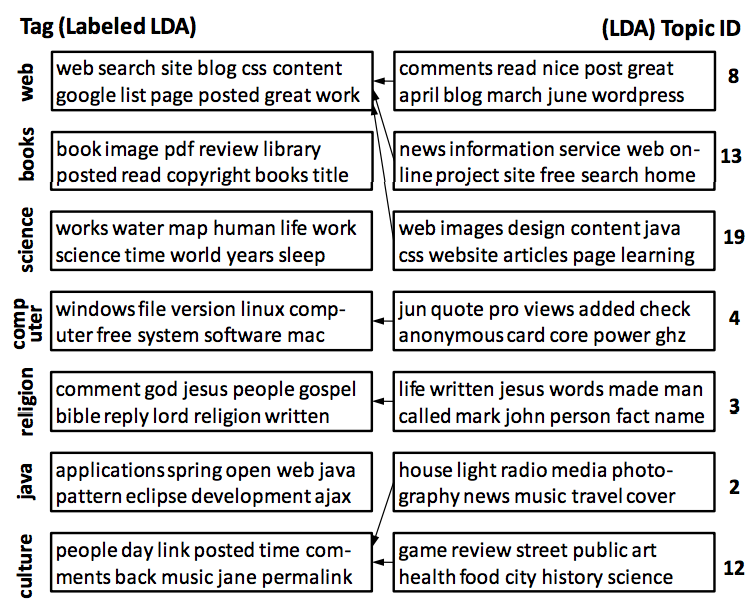
\includegraphics[width=.5\linewidth]{figures/viz_llda}
  \caption{Example of topics learned by labeled \abr{lda} (Figure from
    \citet{ramage-09}).  Each topic in labeled \abr{lda} is associated with a
    label, which encourages the topics to be consistent with the ontology of
    labels.  \abr{lda}, in contrast, uses the empirical frequency of topics to
    divide the dataset, resulting in three topics (8, 13, 19) associated with
    the labeled \abr{lda} \underline{web} topic. }
  \label{fig:llda}
\end{figure}


\section{Displaying Models}

\begin{figure}
  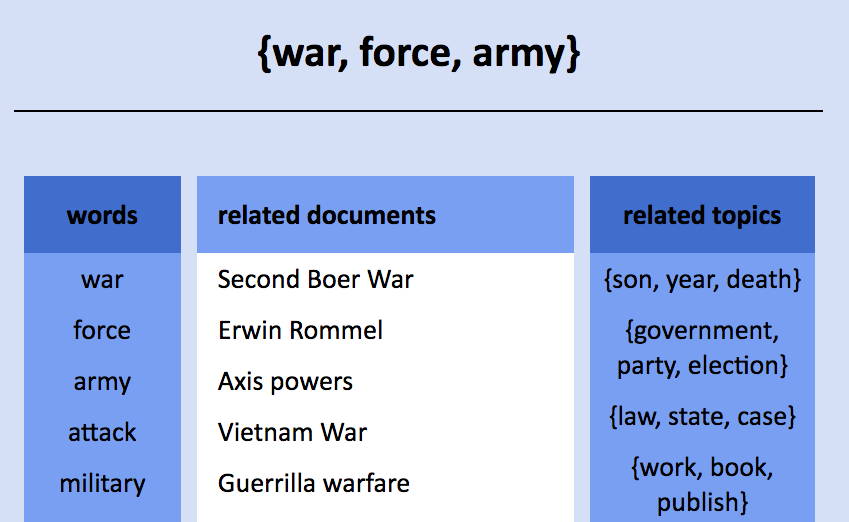
\includegraphics[width=.5\linewidth]{figures/viz_tmve}
  \caption{ }
  \label{fig:llda}
\end{figure}

However, topics are not the end of the story.  Users often want to use topics to
find relevant documents within the collection.  Going back to our example in the
previous chapter, a user may want to find the ``smoking gun'' in the Enron
dataset, not just use topics to understand the main themes in a dataset.

Thus, a good topic model visualization must also show the documents associated
with a topic.  The Topic Model Visualization Engine~\citep{chaney-12} shows the
top documents associated with a topic (Figure~\ref{fig:tmve}).  Recall that each
document has a distribution over topics $\theta_d$, which is a vector with an
entry for each topic.  We focus the dimension associated with a particular topic
and then sort the documents based on that topic coordinate from largest to
smallest.

The topical guide~\citep{gardner-10} extends this approach by enriching topic
views with additional metadata.  For instance, if the collection has dollar
amounts or sentiment~\cite{pang-08} associated with a document, it provides a
histogram of the metadata associated with the topic.  It also provides \emph{in
  context} examples of topic words, allowing to see how a word is used within a
topic (helping to address topic model's bag of words assumptions).

\abr{tome}~\citep{eistenstein-14} focuses on a specific type of metadata: time.
It allows users to view the evolution of topics over time to understand, for
example, how the issue of slavery is reframed from an economic argument to an
argument over human rights.  It supports filtering to specific topics or to see
how words are used over time across topics.

In contrast to showing how topics related to metadata, \citet{chuang-12} focuses
on how topics relate to \emph{each other}.  Their ``Termite'' topic
visualization shows the term-by-term similarity between topics.  By presenting
topic-term probabilities on a grid with topics as the columns and terms as the
rows, users can see when topics share words or when topics are only about a
handful of words.

\begin{figure}
  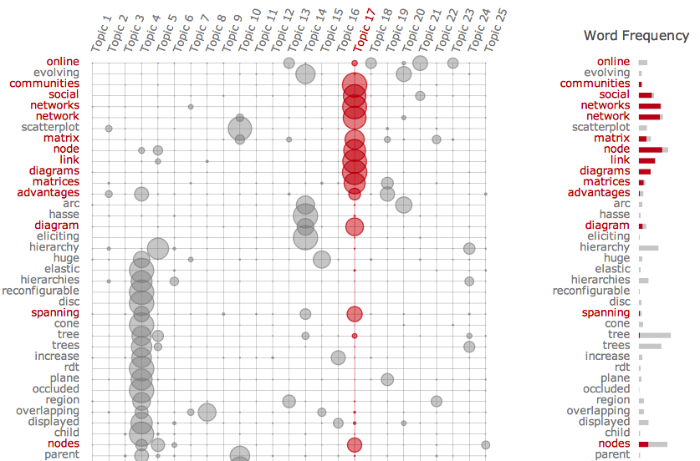
\includegraphics[width=.9\linewidth]{figures/viz_termite}
\end{figure}

\section{Quality, Stability, and Repair}

However, not all topic models are perfect.  \citet{chang-09b} showed that
held-out likelihood, the traditional measure of probabilistic model quality,
emphasizes \emph{complexity} rather than interpretability, what humans
presumably care about.  Thus, automated techniques may not be able to tell you
whether a topic model is good or not.\footnote{Automated
  measurements~\citep{newman-10,mimno-11,lau-14} of topic quality may serve as a
  proxy for human interpretability ratings.}

Visualizations can help show users where topic models have issues.  Showing the
relationships between multiple models can also help distinguish stable from
spurious topics~\citep{chuang-15}, and adjusting the ``hyperparameters'' of
distributions (the Dirichlet parameters of models discussed in Chapter~\ref{})
can have a large effect of what the final models are~\cite{wallach-09b}.

Interactive topic modeling---in conjunction with visualizations---can help
correct the problems of topic models.  A user first get an overview of the
dataset using a visualization of the topics and documents.  Then, the user can
see instances where the model errs and then correct those mistakes.

For example, Figure~\ref{} shows a topic learned from abstracts of grants funded
by the American National Institutes of Health (\abr{nih}).  Most topics were
``good''; they summarized the data and told a story about a coherent slice of
research supported by the \abr{nih}.  However, this topic is more problematic;
it combines words about the central nervous system with words about the urinary
system.  Such a topic (as discussed in \citet{}) does not give a clear
understanding of the documents it should represent.

\citet{hu-14:itm} address this problem by allowing a user to add probabilistic
constraints to the model~\citep{boyd-graber-07,andrzejewski-09}.  For example,
the user might say that ``bladder'' and ``spinal cord'' don't belong in the same
topic together.  Figure~\ref{} shows how the topic is more focused after the
user provides this feedback.  In contrast to probabilistic constraints,
\citet{choo-13} add matrix factorization constraints, which are in practice much
faster.

\section{Conclusion}

Much of what topic models are used for is to help users understand corpora.
However, the output of topic models don't give insights to users without the
helpmeet of interactive visualizations which allow users to discover and
refine insights.  In the next chapters we'll talk about specific applications of
these insights, but these insights are often built on the initial understanding
of a model offered by the visualizations discussed in this chapter.